\documentclass[a4paper,10pt]{article}

\usepackage[margin=2cm]{geometry}
\usepackage{graphicx}
\usepackage{amsmath}
\usepackage{array}
\usepackage{hyperref}
\usepackage[all]{hypcap}
\usepackage{listings}
\lstdefinestyle{TerminalStyle}{
  language=bash,
  basicstyle=\small\sffamily,
  numbers=left,
  numberstyle=\tiny,
  numbersep=3pt,
  frame=tb,
  columns=fullflexible,
  linewidth=0.9\linewidth,
  xleftmargin=0.1\linewidth
}
\lstdefinestyle{HtmlStyle}{
  language=html,
  basicstyle=\small\sffamily,
  numbers=left,
  numberstyle=\tiny,
  numbersep=3pt,
  frame=tb,
  columns=fullflexible,
  linewidth=0.9\linewidth,
  xleftmargin=0.1\linewidth
}
\lstdefinestyle{OutputStyle}{
  language=html,
  basicstyle=\small\sffamily,
  frame=tb,
  columns=fullflexible,
  linewidth=0.9\linewidth,
  xleftmargin=0.1\linewidth
}

\setlength{\parindent}{0pt}
\setlength{\parskip}{1ex plus 0.5ex minus 0.2ex}
\title{
\includegraphics[width=12cm]{Eeufeeslogo.jpg} \\
       Department of Computer Science \\
       University of Pretoria \\
       \vspace{0.5cm}
       Software Engineering\\
       COS301 Main Project \\
       \vspace{1.0cm}
       \begin{large} \textbf{Team CodeX}\\ ReRoute Purchasing Management Systems\end{large}\\
       \vspace{1.0cm}
       User Manual \\}
       
\date{August 10, 2017} 
\author{}

\begin{document}
\maketitle
\thispagestyle{empty}
\clearpage

\newpage
\pagenumbering{roman}
\thispagestyle{empty}
\tableofcontents
\clearpage

\newpage
\pagenumbering{arabic}

\section{Introduction}
Reroute Systems is a software company with different in-house developed applications. The Purchase Management System 
application specifically, is the main application and mainly active in the pharmaceutical space.\\
This document contains guidelines on how the application works, and how one can maximise the application and all it entails for best use.\\

\section{General Information}
\subsection{Title Page}
This application is the Reroute Purchasing Management System affiliated with the Reroute Systems company.\

For best use, it is advised that users have background knowledge in the pharmaceutical space.\\

\subsection{System Overview}
The system is a search engine called \textbf{Smart Search Pharmaceutical} which is enriched with functionality. Our system allows the user to customize how the search alorithm relates words to eachother. This allows the user to search for a term as well as terms related to it, different spellings and different variations of the term. Our system allows the users to retrieve specific records from very large amounts of data in a very small amount of time. 

	\subsubsection{Stakeholders}
	The stakeholders of the system include the following:
	\begin{itemize}
	\item \textbf{The Client} is Diederik Mostert, Software Director of ReRoute Systems who proposed the project as a result of a challenge faced in the company, which is to search a product on master file with different combination used by each wholesaler.
	\item \textbf{Users in Pharmaceutical space} They will use the system to retrieve information of the product they need.
	\end{itemize}
\subsection{System Configuration}
	{\centering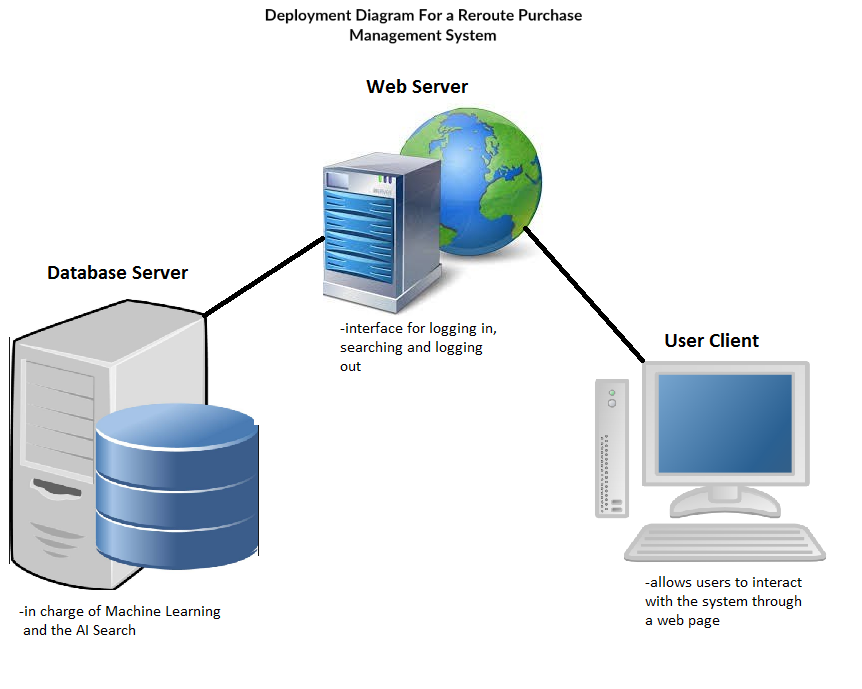
\includegraphics[width=15cm, scale=0.5]{User Manual Deployment diagram.png}} \\

\subsection{Note to the User}
This system allows the user to search for a word and related terms. It also allows the user to link words to eachother. This allow the user to customize their experience to their needs. For example, the user can link words like Panado to Grandpas or headache so that if you were to search Headache you will also receive the results for Panado's and Grandpas. This is made possible through the use of a dictionary. To get the ultimate experience, it is advised that the user make use of this dictionary by linking terms they wish to be linked.

\subsection{Installation}
To be implemented.

\section{Getting started}
	The application design looks as follows: \\
	\subsection{Main screen}
	When the app is launched it requires your login credentials.\\
	{\centering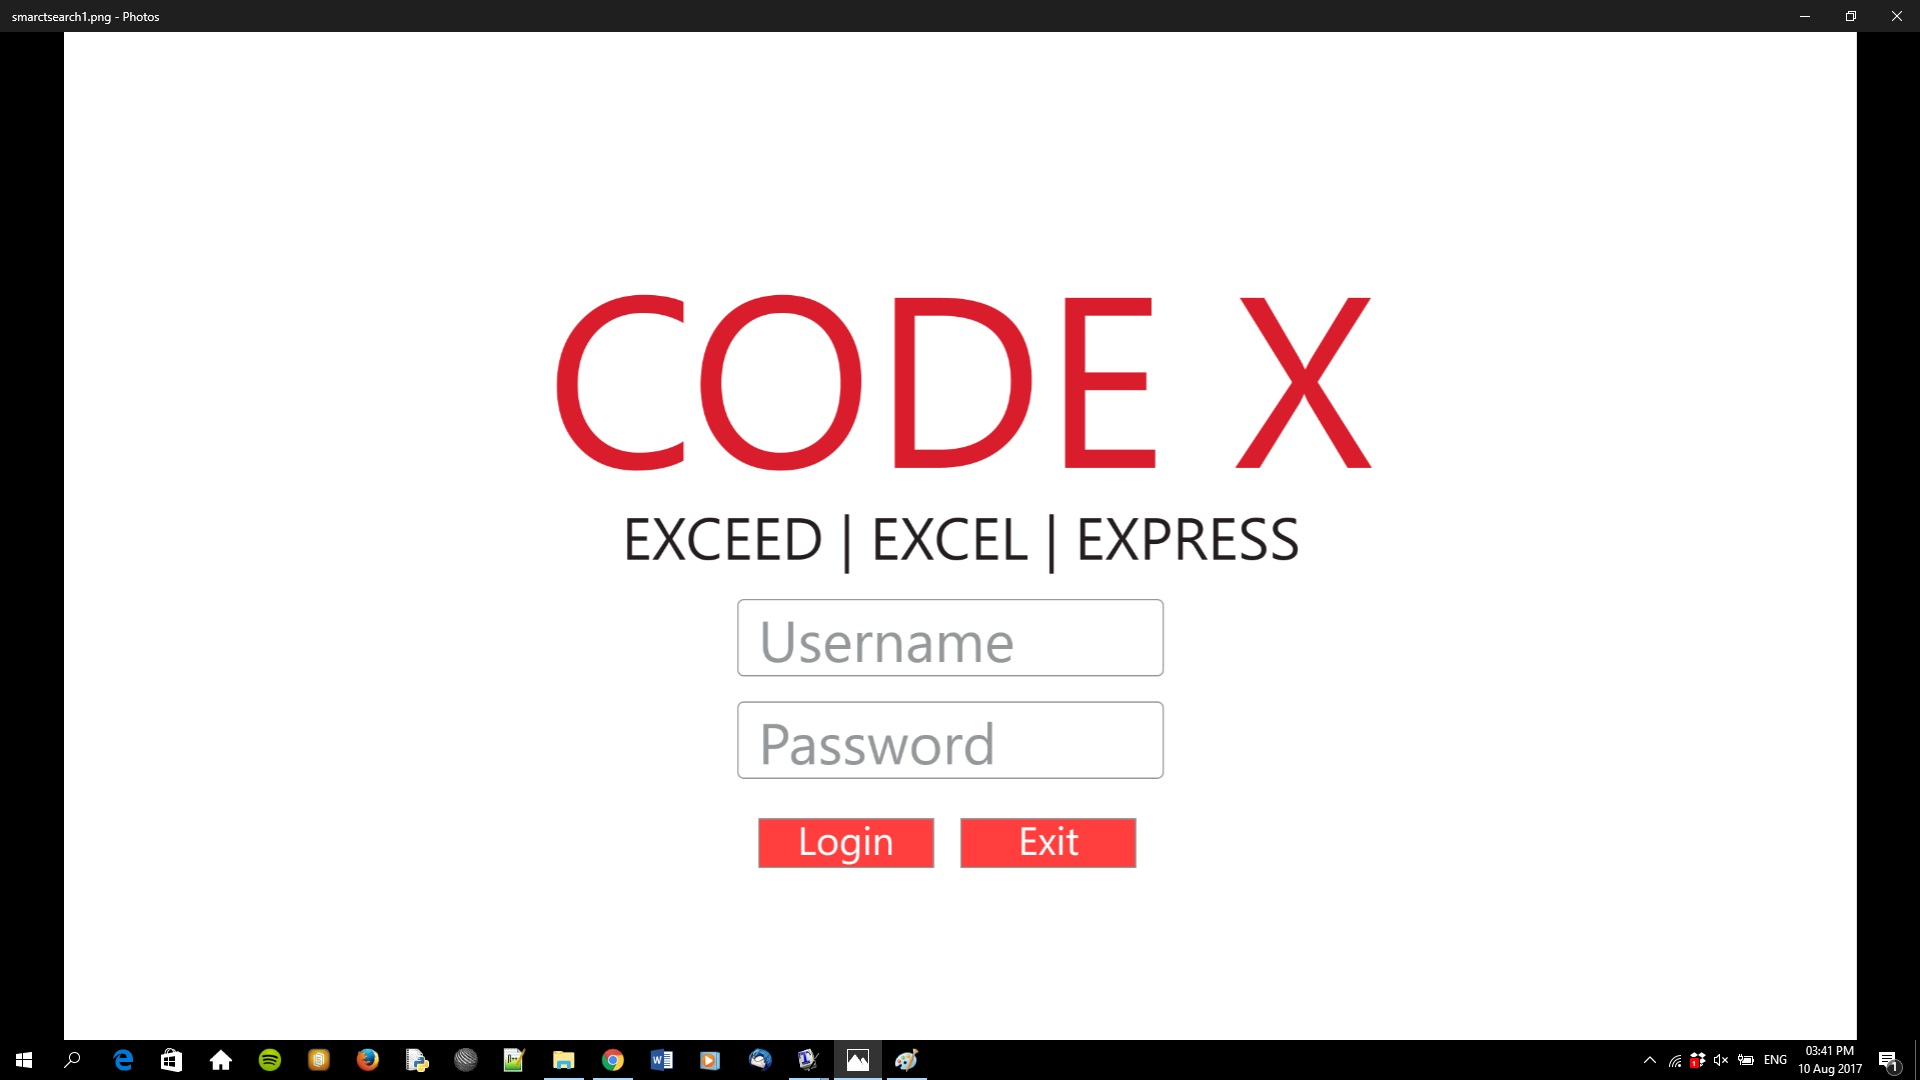
\includegraphics[width=15cm, scale=0.5]{smarctsearch1.jpg}}
	\subsection{Pharmaceutical Search Menu}
	The search screen where the user enters the product information to search on. \\
	{\centering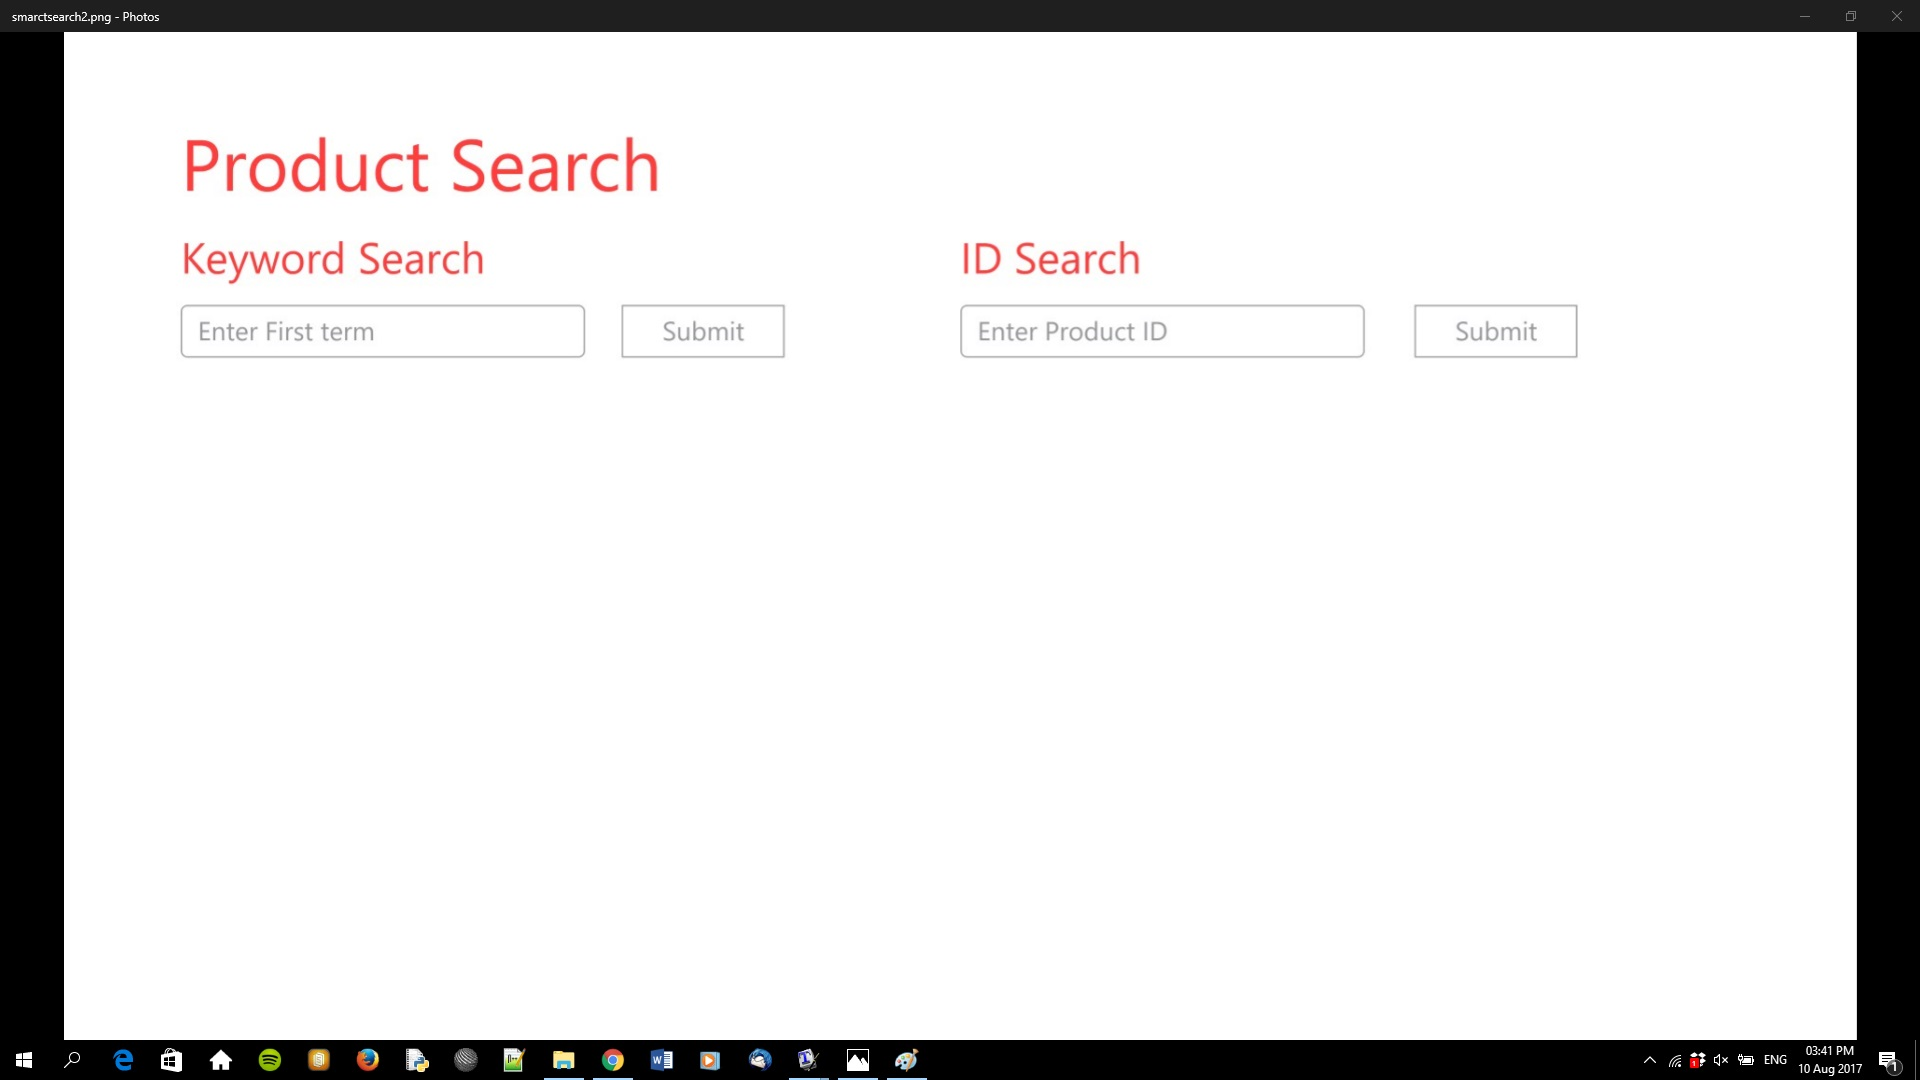
\includegraphics[width=15cm, scale=0.5]{smarctsearch2.jpg}} \\ \\
	{\centering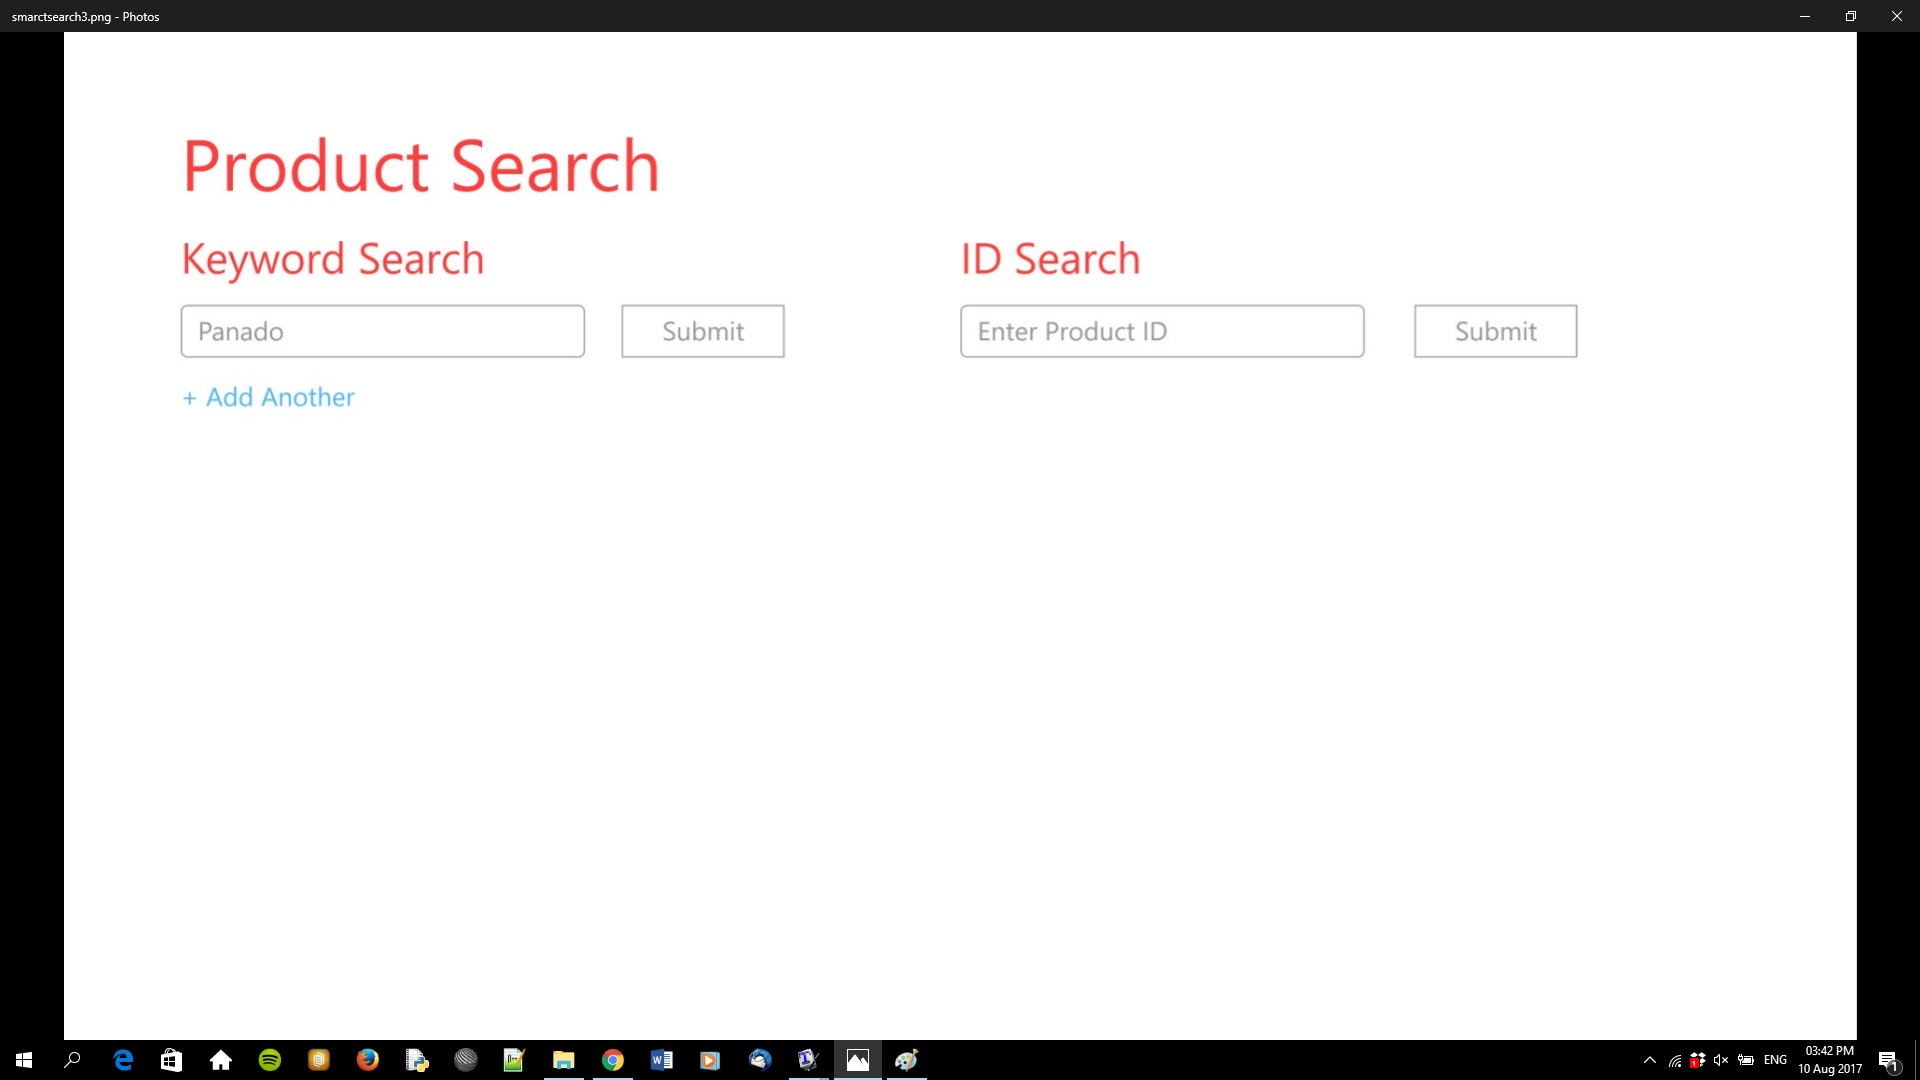
\includegraphics[width=15cm, scale=0.5]{smarctsearch3.jpg}} \\ \\
	{\centering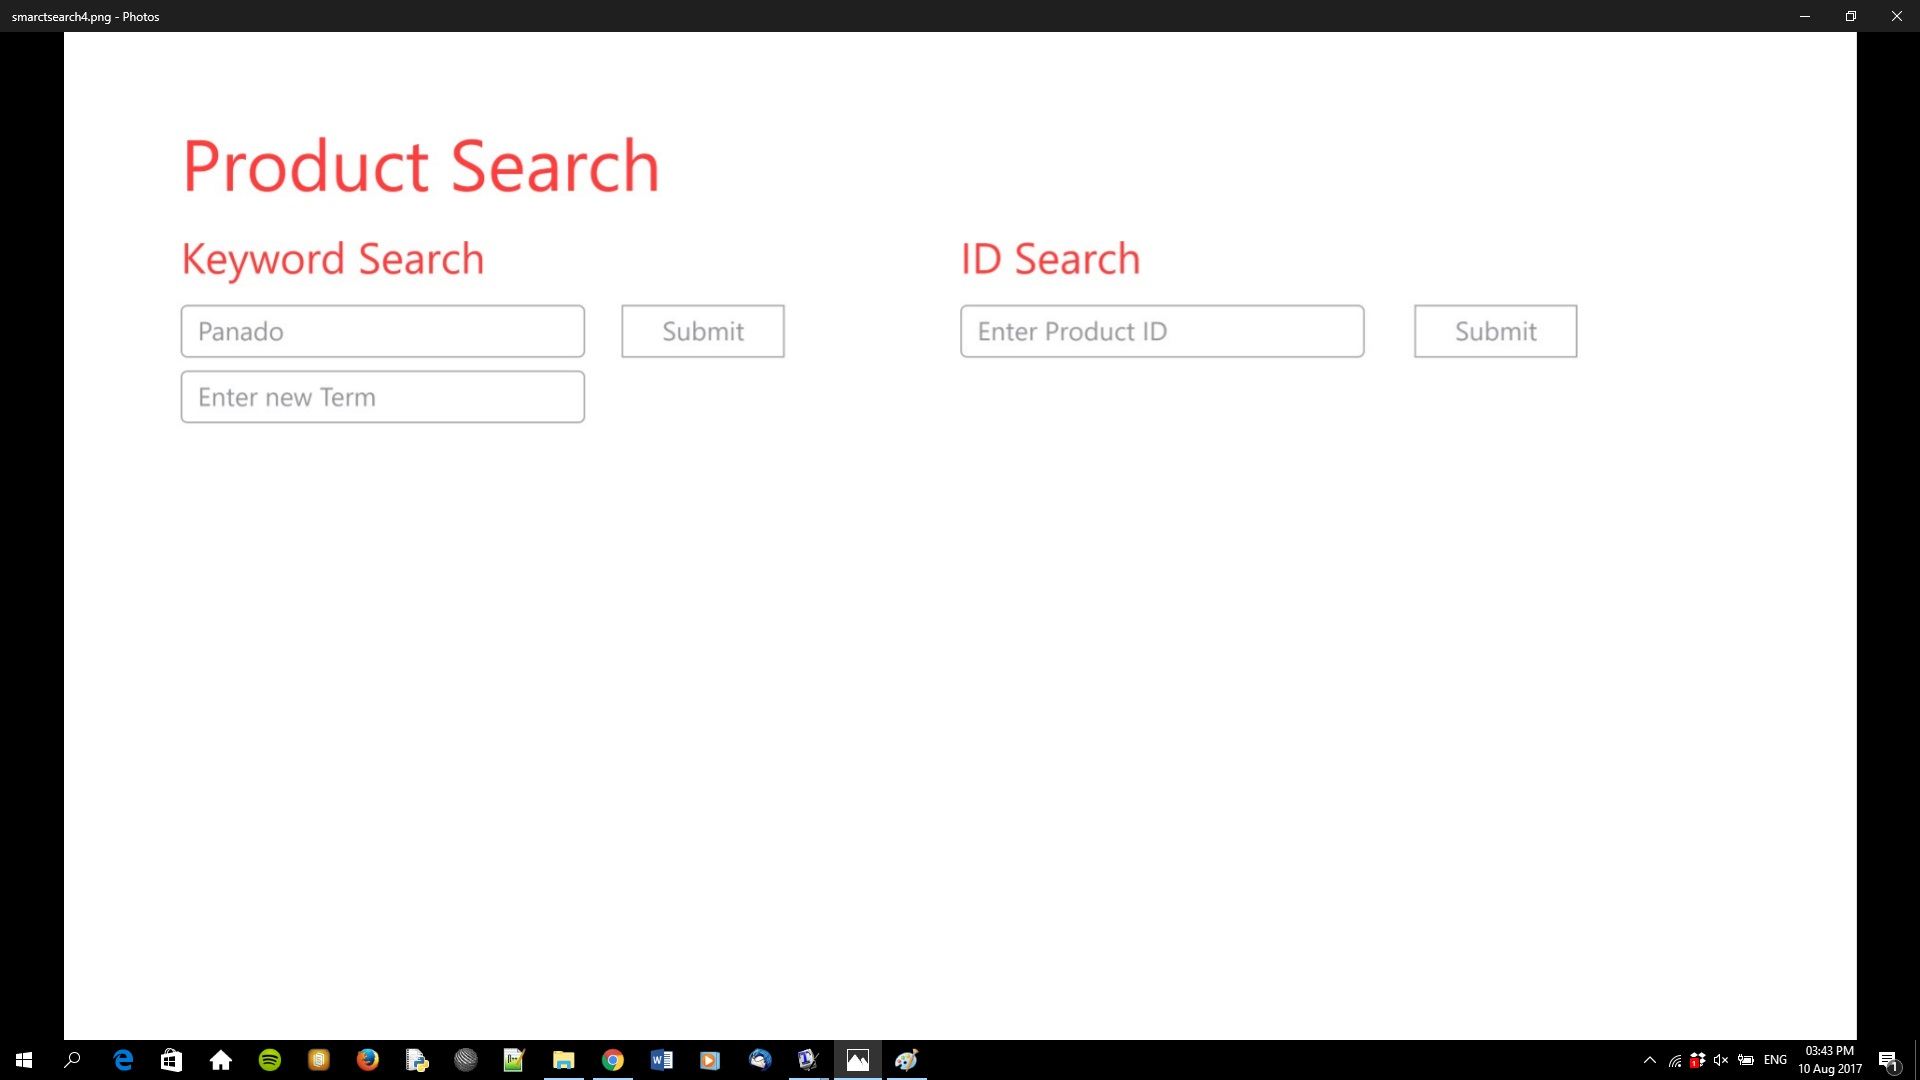
\includegraphics[width=15cm, scale=0.5]{smarctsearch4.jpg}} \\ \\
	{\centering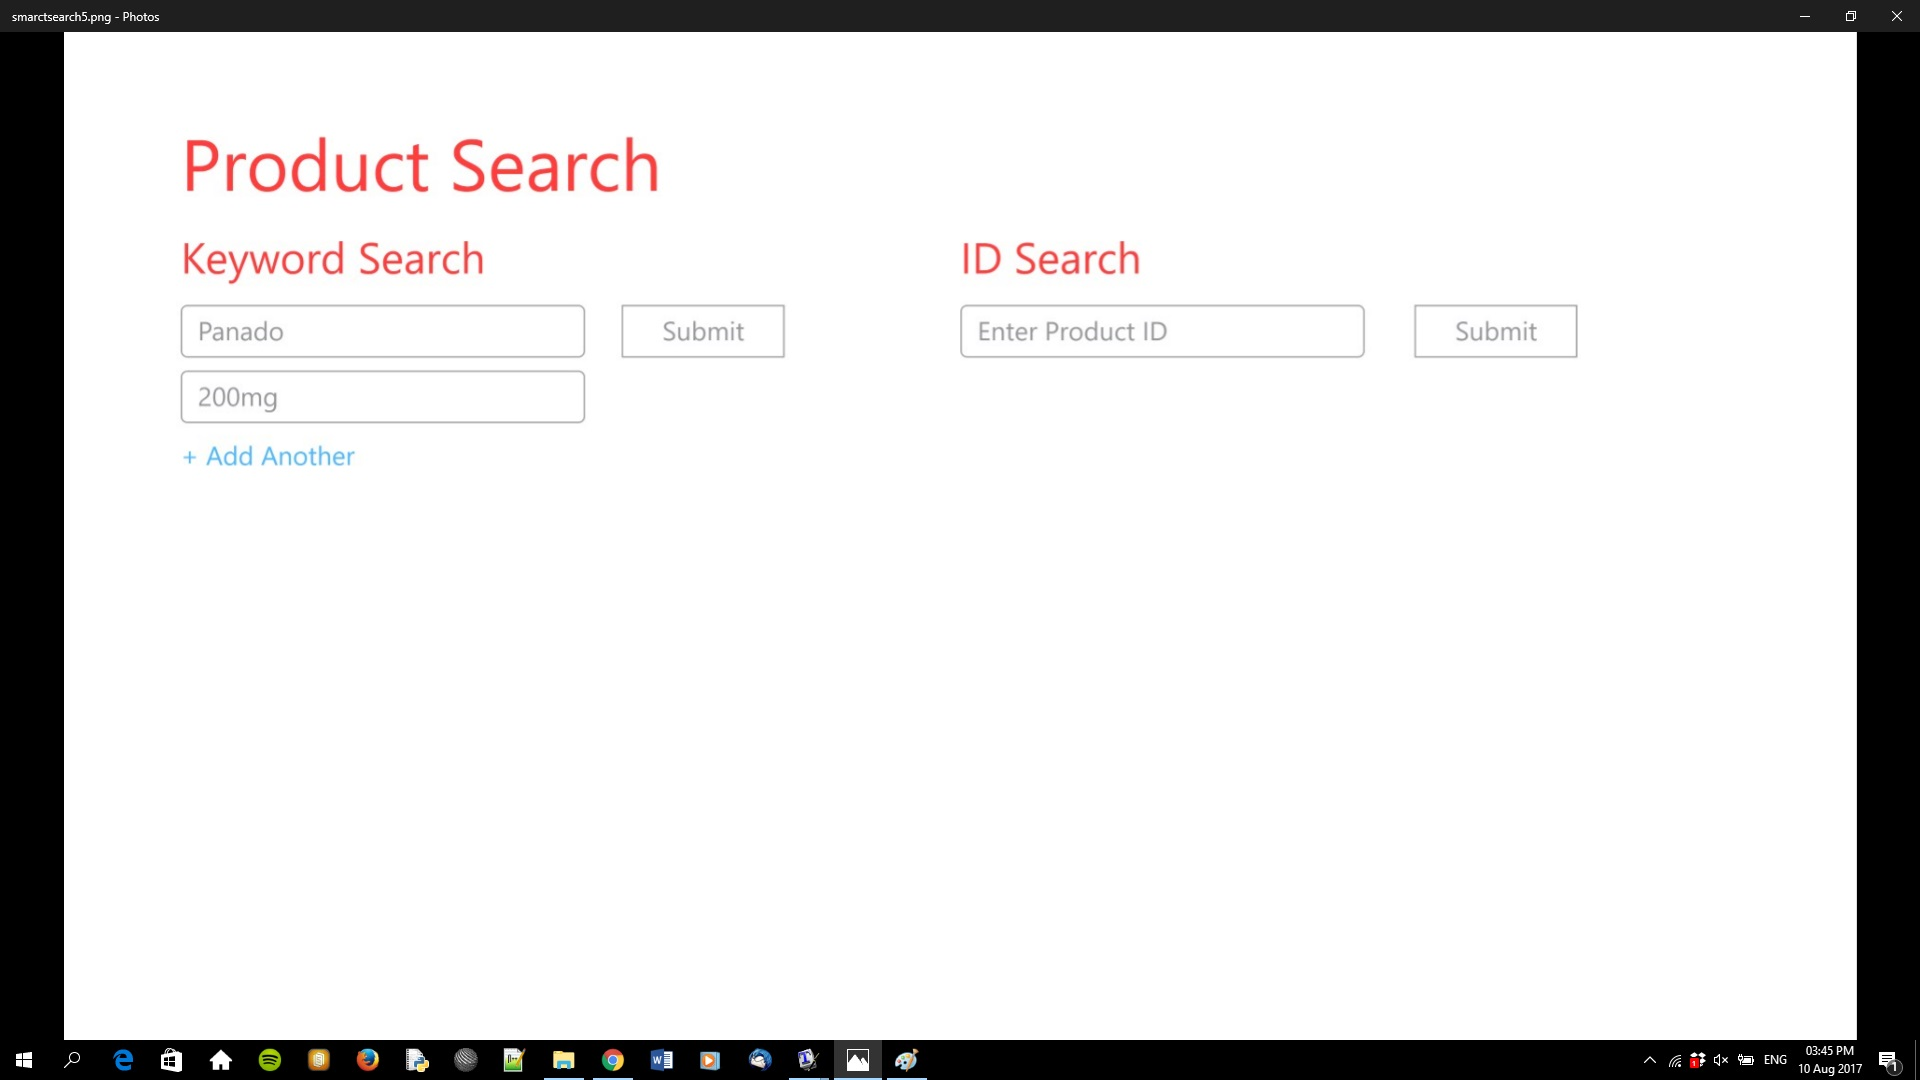
\includegraphics[width=15cm, scale=0.5]{smarctsearch5.jpg}} \\
	\subsection{Search result}
	The result of a search would yield a result below: \\
	{\centering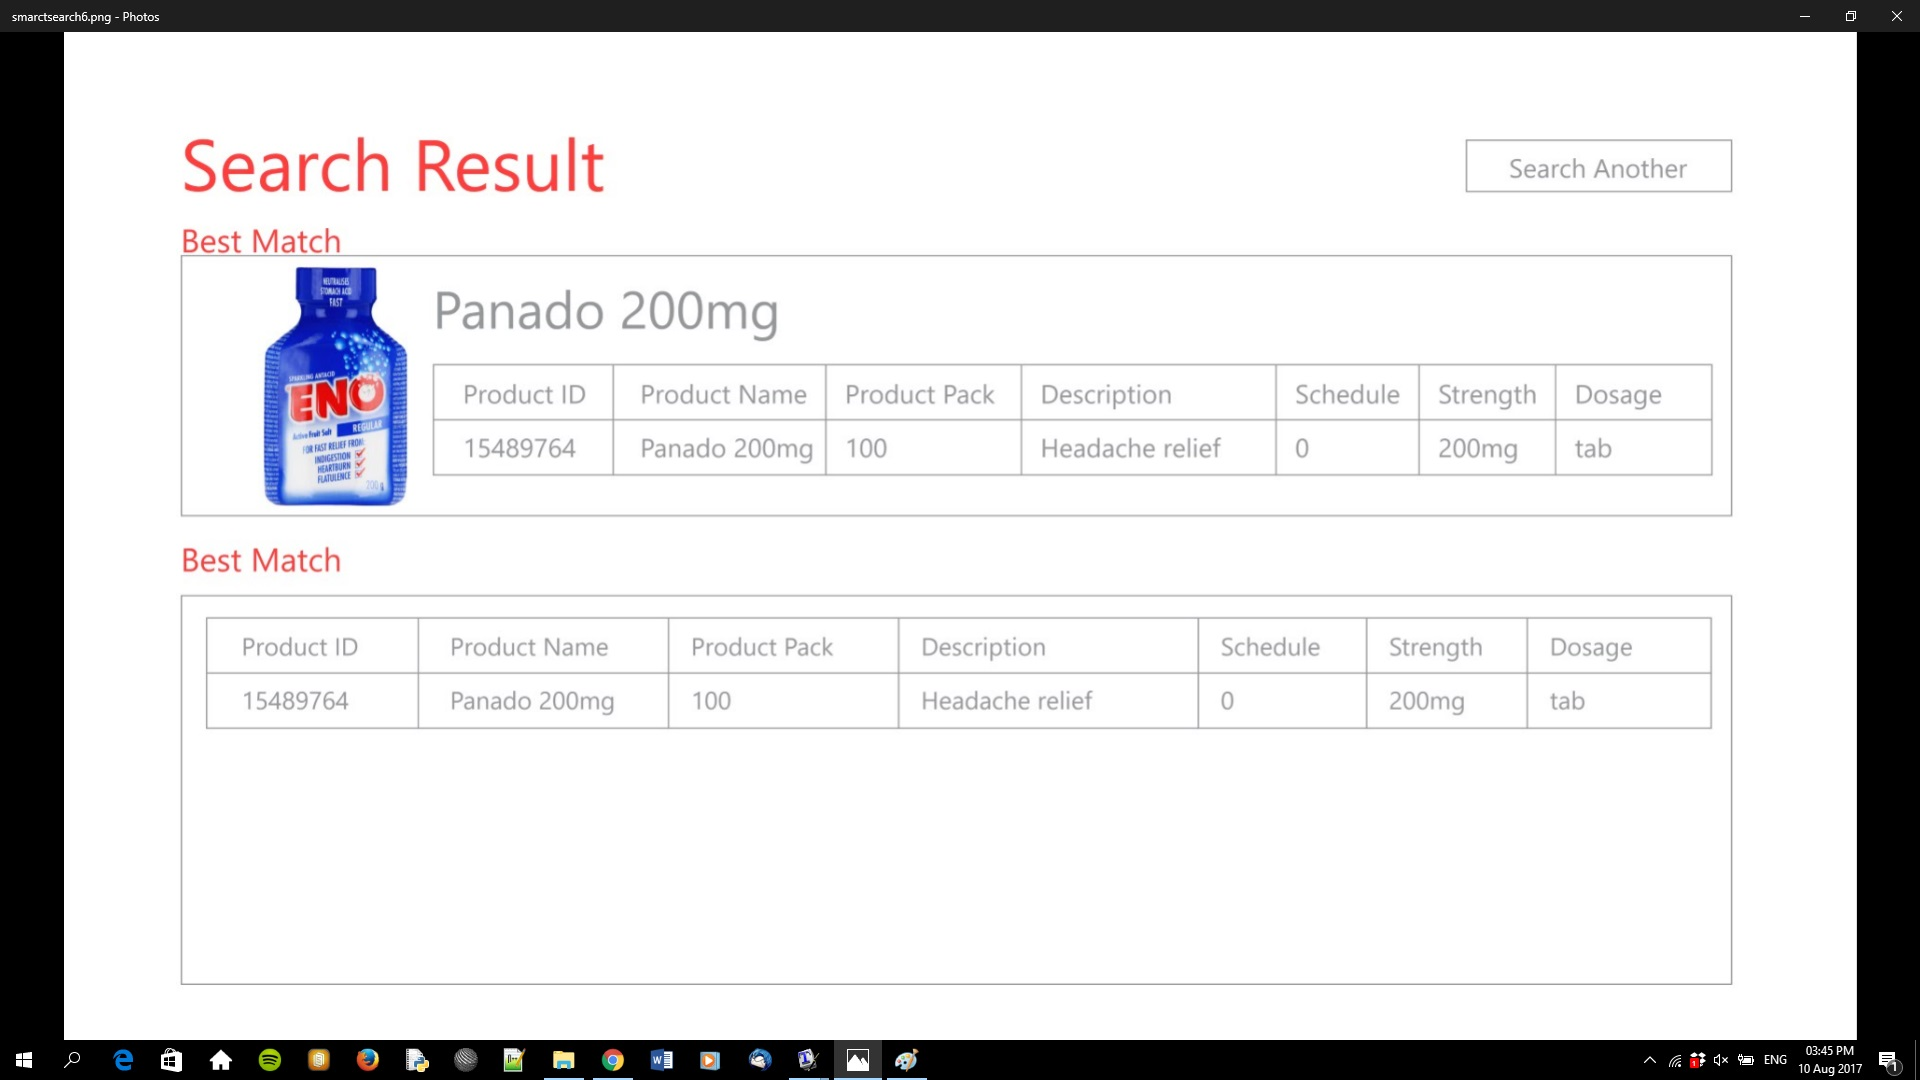
\includegraphics[width=15cm, scale=0.5]{smarctsearch6.jpg}} \\
	
\section{Using the system}
	After registering yourself as a user, you can use the following actions to use the system:
	\begin{enumerate}
	\item Logging In:
		After running the program, you will be presented with a login screen.  In this screen, you will need to provide your username and password to gain access to your account.
	\item Menu:
		After logging in, you will be presented with a screen containing the different options a user can take. These options are (1) Search, (2) Edit Dictionary, (3) Dictionary, and (4) Delete Record.

	\item Search:
		At this screen you will be presented with an option to search a product by name or by ID. If you would like to search by name, type the name or something related to it, and press the search button. If you would like to search by ID you need to type the exact ID and then press search.  After pressing search, you will be presented with either possible matches to your search or the exact match to the ID.  From here you can select products you are interested to order.
	\item Edit Dictionary
		At the Edit dictionary screen you can see the words already added to the dictionary. Here you can delete words that you would prefer not to be linked at all.
	\item View Dictionary
		At the Dictionary sceen you can add words to the dictionary that you would like to be linked. For example, you can link the word tabs to tablets by inserting the word tabs in the left text box and the word tablets in the right text box. These words will now be linked and both will be included in the result when searched for. 
	\item Delete Record
		At this option the user can delete data from the tables. 
	\item Logout:
		After placing an order and have no more to do, remember to logout. To do so, simply press the logout button.\\
	\end{enumerate}
\section{Troubleshooting}
	Please report any errors found with this system to allow development teams to correct it. If you wish to do so yourself, here are some useful things to look at:

	\begin{enumerate}
		\item General Issues
			Most issues can be fixed by simply restarting the program or your computer. 
		\item Error communicating to the database
			The database system we use, zizo, makes use of SOAP and REST calls to communicate with the rest of the system. Esure that the system has internet connection. If you do have internet connection, ensure that the system is commmunicating with the database system. 
		\item System crashes
			Please report any areas or actions that cause the system to crash to the developers.
		\item Faulty data
			Reading data into the database is an automated process and faulty data often get through. Please report such cases to Rerout Systems.
	\end{enumerate}
	

\end{document}
